\documentclass{article}

\usepackage{graphicx}
\usepackage[font=small,labelfont=bf]{caption} % Required for specifying captions to tables and figures
\usepackage{hyperref}
\hypersetup{
    colorlinks,
    citecolor=black,
    filecolor=black,
    linkcolor=black,
    urlcolor=black
}

\graphicspath{{assets/}} % images in /assets/ folder

\title{Digital Logic Design Project 2} % Sets article title
\author{Zidane Karim} % Sets authors name
\date{\today} % Sets date for date compiled

% The preamble ends with the command \begin{document}
\begin{document} % All begin commands must be paired with an end command somewhere
    \maketitle % creates title using information in preamble (title, author, date)
    \tableofcontents

    \section{Introduction} % creates a section
    
        
    The assignment was to design a sequential logic circuit that can both write and read a byte into a RAM chip, to be displayed on an array of LED outputs. 
    
    In other words, the circuit should be able to take in an 8-bit input and store it in memory, and then be able to read that memory and display it on the LED array.
    
    For example, if the input is 10101000, the LED array should display the following configuration: $\downarrow$

    \begin{center}
        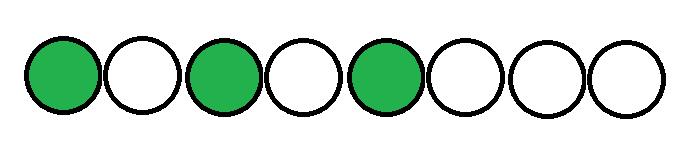
\includegraphics[width=0.5\textwidth]{LED_Output_Paint.png}
        \captionof{figure}{LED Output for 10101000}
    \end{center}

    The heart of the problem is manipulating the data around the RAM chip, as it was a 1024$\times$4 RAM chip, meaning it had 1024 memory locations, each with 4 bits of data.
    
    However, recall that the input is 8 bits, so we need to split the input into two 4-bit chunks to store in the RAM chip.
    
    The circuit should be able to write the first 4 bits into the RAM chip, and then write the second 4 bits into the RAM chip, and then read the data from the RAM chip and display it on the LED array.
    
    This manipulation of data is the main challenge of the project, which is why we turn to a sequential finite state machine to solve the problem.

    \subsection{Outline}
        \subsubsection{Methodology}

        The circuit is divided into three main parts: the input, the RAM chip, and the output.
        The essential issue in each was:
        \begin{itemize}
            \item Input: Automatically splitting the 8-bit input into two 4-bit chunks to write to the RAM chip in sequence 
            \item RAM Chip: Keeping the data in memory and being able to read it back out without losing it/moments of gibberish
            \item Output: Continously displaying the data on the LED array
        \end{itemize}
        \subsubsection{Implementation}
        The vast majority of the circuit was implemented using TTL chips. The only exception was the bidirectional register used to hold the data which was a CMOS chip, requiring additional buffering.

    \section{Methods}
        \subsubsection{Theory}
        The circuit was designed as two finite state machines, one for read and one for write:
        \begin{itemize}
            \item The \textbf{write FSM} would take in the 8-bit input and split it into two 4-bit chunks, writing them to the RAM chip in sequence.
            \item The \textbf{read FSM} would read the data from the RAM chip and display it on the LED array.
        \end{itemize}
            
        \textbf{Why do we use a finite state machine?}\\ 
        
        Because the circuit needs to be able to remember the state it is in, and then change states based on the input. This is the essence of a finite state machine.
        The practical relation to the circuit is that the circuit needs to know whether it is in the write state or the read state, and then change addresses in the RAM chip accordingly.
        based on the details of the state. 

        This comes from the fact that the RAM chip has a limited address width (10 bits for 1024 locations), which requires control over address selection to store and retrieve the data correctly.

        In addition to addresses, the RAM chip requires a write-enable signal to write data to memory. This signal is controlled by the write FSM, which is responsible for writing the data to the RAM chip in the correct sequence.

        The design of the RAM chip has certain time-intervals where between address changes, the data written to memory is invalid/incorect. Because of this, the write FSM must be designed to wait for the correct time to write the data to memory, and then change the address to write the next data.

        However, the timing intervals on the 2114 TTL RAM chip is measured in nanoseconds, which our clocks generated from 555-timers cannot feasibly reach due to equipment availability. Thus, this timing was not of much concern considering our RAM chip would never be able to reach the speeds required to cause a problem. 
        Because of this, we do not really care about an idle state in both FSMs as the RAM chip will never be able to write/read data fast enough to cause a problem. But in my original thinking, I designed the states with an idle in mind.\\~\\

        

        To summarize, the finite state machines are responsible for selecting the correct address and enabling the read or write operation as required by the process:
        
        \textbf{Why do we use external registers?}\\ 

        The RAM chip has a 4-bit data width, which means it can only store 4 bits of data at a time. However, the input is 8 bits, which means we need to split the input into two 4-bit chunks to store in memory.

        To do this, we use two 4-bit registers to hold the data before writing it to memory. The first register holds the first 4 bits of data, and the second register holds the second 4 bits of data.
        Why do we use registers instead of reading from RAM directly?\\

        This is because the RAM chip has a limited address width, which means we need to write the data to memory in the correct sequence. If we read the data from memory directly, we would not be able to control the sequence in which the data is written to memory.
        In other words, we want to view all the data at once, not just the 4-bits at a time. The external registers also store the values inside so we can change the values on the dip switches, yet the values on the LED array remain the same since we have not written to the RAM.\\ 

        \subsubsection{State Transitions and Truth Tables}
        
        \begin{center}
            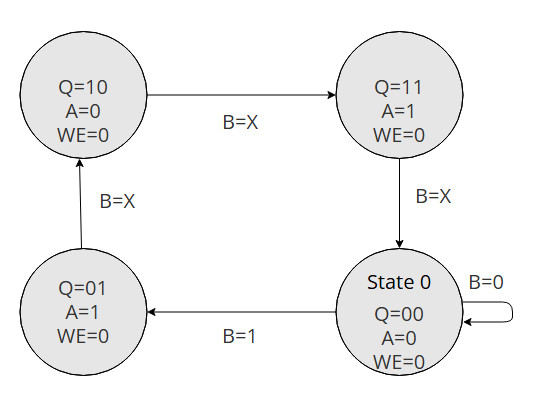
\includegraphics[width=0.5\textwidth]{READ_State_Transition.png}
            \captionof{figure}{Read State Transition Diagram}
            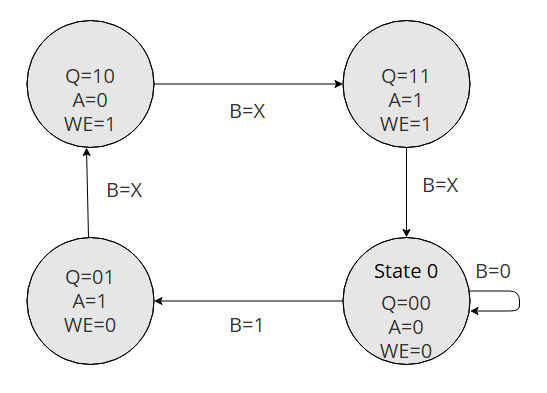
\includegraphics[width=0.5\textwidth]{WRITE_State_Transition.png}
            \captionof{figure}{Write State Transition Diagram}        
        \end{center}

        Above are the two state transiton diagrams for read and write respectively. Notice that they almost exactly the same, except the write FSM uses the write enable signal to write to memory, while the read FSM leaves it off the entire time.
        These FSMs are Mealy Machines as outputs rely on the button presses as well as the original states. The essential logic of both FSMs is to stay idle until the button is pressed, which then cycles through the diagram. At each point, the machine switches addresses and either writes or reads.\\ 

        Below is the truth table for the FSMs, which is used to create the Karnaugh Maps for the FSMs. The truth table is the same for both FSMs, except the write FSM has an additional output for the write enable signal.    
        From this, we can derive logical expressions and then simplify them to create the FSM circuits.\\
        \begin{minipage}{\textwidth}
            \begin{center}
            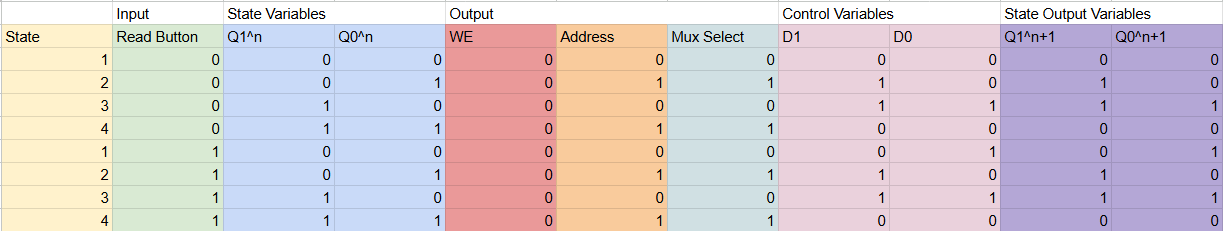
\includegraphics[width=1.2\textwidth]{READ_Truth_Table.png}
            \captionof{figure}{Read Truth Table}
            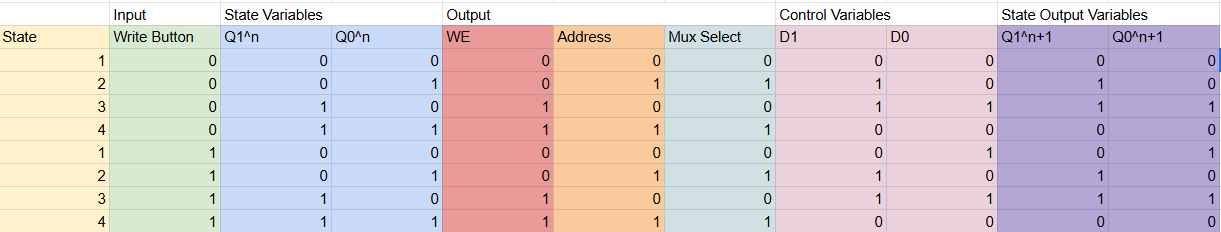
\includegraphics[width=1.2\textwidth]{WRITE_Truth_Table.png}
            \captionof{figure}{Write Truth Table}        
            \end{center}
        \end{minipage}

        \subsubsection{Boolean Expressions}
        \begin{minipage}{\textwidth}
            \begin{center}
            %d1 = q1 xor q0
            %d0 = RB or Q1 * !Q0
            Read: 
            \begin{itemize}
                \item \( D_1 = Q_1 \oplus Q_0 \)
                \item \( D_0 = (R_B + Q_1) \cdot \overline{Q_0} \)
                \item \( OE = \overline{WE} \)
            \end{itemize}
            Write:
            \begin{itemize}
                \item \( D_1 = Q_1 \oplus Q_0 \)
                \item \( D_0 = (W_B + Q_1) \cdot \overline{Q_0} \)
                \item \( WE = Q_1\)
            \end{itemize}
            Both:
            \begin{itemize}
                \item \( A_0 = Q_0R + Q_0W \)
                \item \( Mux Select =  Q_0R + Q_0W \)
            \end{itemize}


            \end{center}

        The tri-state buffer controllers are connected to the write enable signal, because logically the RAM should only receive the inputs when write enable is on.\\\\
        The mux select is connected to the address signal, because we want to select the proper address from the mux based on the state of the FSM.\\\\
        Output enable does not actually exist on the RAM chip but it does in Logisim. It is connected to the inversion write enable signal, because we only want to read the data when the write enable signal is off.
        Since WE is off by default, when we are not writing, we are reading. \\\\
        The final puzzle to solve is the register clock. The register is not hooked up to the 555-timer clock, because then it would read on every clock, which we do not want. We only want to update the register's value to the LED when we press the read button.
        Since the \(Q_0\) of Read controls the address, we can connect the output of \(Q_0\) to the first register and the inversion/negation of this signal to the other register. This way, when we press the read button, the register will update to the value of the LED array.\\ 
        
        \end{minipage}

        \subsubsection{Functional Block Diagrams}
        \begin{center}
            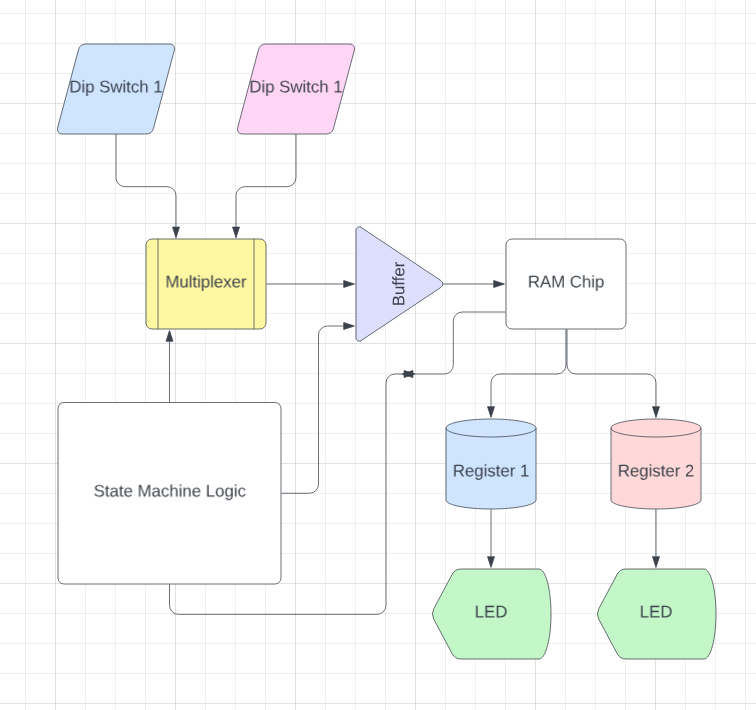
\includegraphics[width=1\textwidth]{FunctionalDiagram.png}
            \captionof{figure}{Functional Block Diagram}
        This follows the logic of the entire circuit. The input is split into two 4-bit chunks, which are then written to the RAM chip. The RAM chip is then read and displayed on the LED array through storage on the registers.\\
        \end{center}

        \subsubsection{Logic Diagrams}

        \begin{center}
            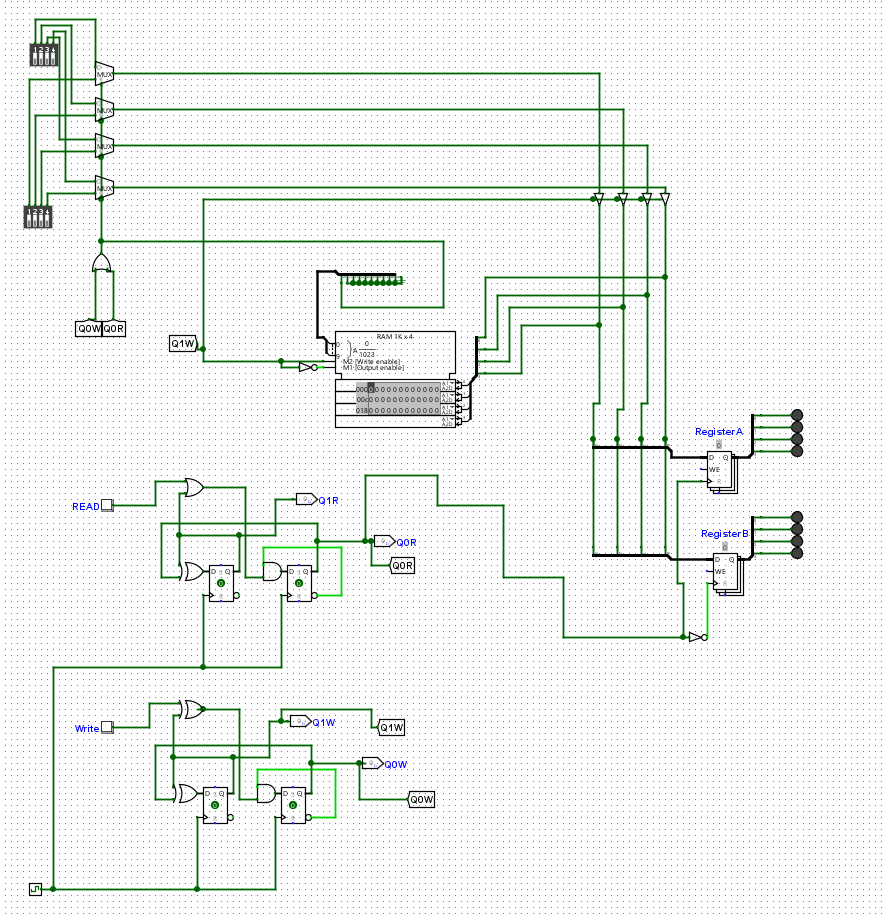
\includegraphics[width=1\textwidth]{Circuit.png}
            \captionof{figure}{Entire Circuit}
            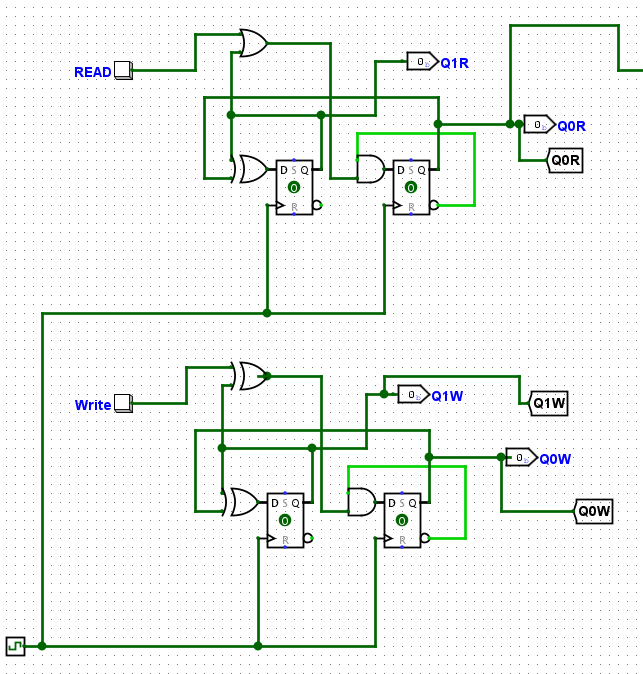
\includegraphics[width=1\textwidth]{FSM_Circuits.png}
            \captionof{figure}{Read and Write FSM Circuits}
            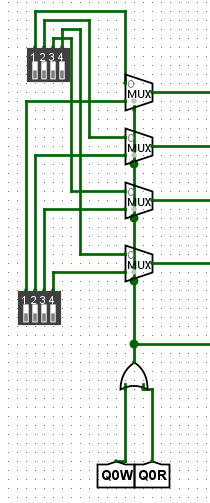
\includegraphics[width=0.5\textwidth]{muxes.png}
            \captionof{figure}{Muxes and Inputs}
            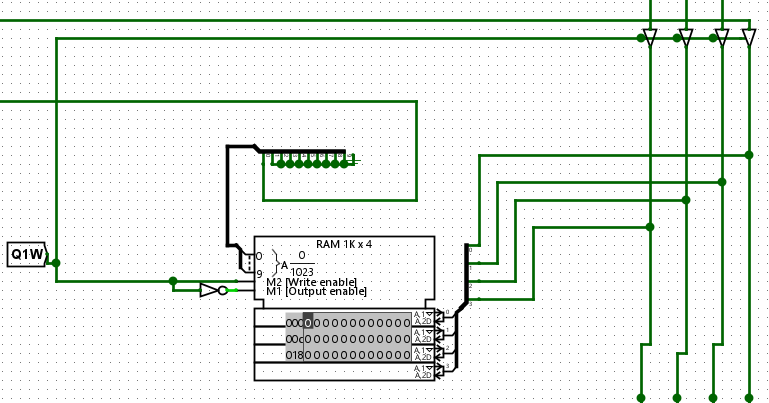
\includegraphics[width=1\textwidth]{RAM.png}
            \captionof{figure}{RAM Chip}
            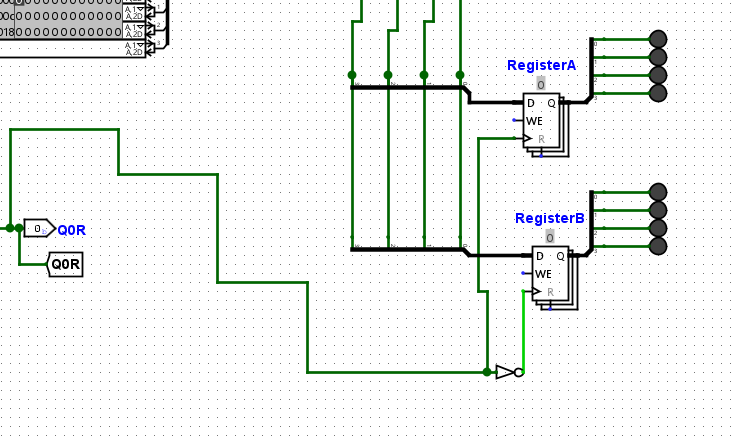
\includegraphics[width=1\textwidth]{Register.png}\
            \captionof{figure}{Registers and Outputs}
        \end{center}
        
        
    \section{Implementation}  
        \subsubsection{TTL-CMOS Interfacing}

        
    

        \subsubsection{Components}
        The circuit was implemented using the following components:
        \begin{itemize}
            \item 74LS161 4-bit counter
            \item 74LS32 Quad OR gate
            \item 74LS86 Quad XOR gate
            \item 74LS00 Quad NAND gate
            \item 74LS08 Quad AND gate
            \item 74LS04 Hex inverter
            \item 74LS139 Dual 2-to-4 decoder
            \item 74
            \item \\
        \end{itemize}

\end{document} % This is the end of the document